% ****** Start of file aipsamp.tex ******
%
%   This file is part of the AIP files in the AIP distribution for REVTeX 4.
%   Version 4.1 of REVTeX, October 2009
%
%   Copyright (c) 2009 American Institute of Physics.
%
%   See the AIP README file for restrictions and more information.
%
% TeX'ing this file requires that you have AMS-LaTeX 2.0 installed
% as well as the rest of the prerequisites for REVTeX 4.1
% 
% It also requires running BibTeX. The commands are as follows:
%
%  1)  latex  aipsamp
%  2)  bibtex aipsamp
%  3)  latex  aipsamp
%  4)  latex  aipsamp
%
% Use this file as a source of example code for your aip document.
% Use the file aiptemplate.tex as a template for your document.
\documentclass[%
 aip,
% jmp,
% bmf,
% sd,
% rsi,
 amsmath,amssymb,
%preprint,%
 reprint, floatfix%
%author-year,%
%author-numerical,%
% Conference Proceedings
]{revtex4-1}

\usepackage{graphicx}% Include figure files
\usepackage{dcolumn}% Align table columns on decimal point
\usepackage{bm}% bold math
%\usepackage[mathlines]{lineno}% Enable numbering of text and display math
%\linenumbers\relax % Commence numbering lines

\usepackage[utf8]{inputenc}
\usepackage[T1]{fontenc}
\usepackage{mathptmx}
\usepackage{mathtools}
\usepackage{etoolbox}
\usepackage{booktabs}
\usepackage{multirow}
\usepackage{subcaption}
\usepackage{gensymb}
\usepackage{siunitx}
\usepackage[version=4]{mhchem}
\usepackage{bm}
\DeclareSIUnit\gauss{G}
\DeclareSIUnit{\angstrom}{\textup{\AA}}
\usepackage[hidelinks]{hyperref}
\hypersetup{
    colorlinks=true,
    linkcolor=blue,
    filecolor=magenta,      
    urlcolor=cyan,
    pdftitle={Overleaf Example},
    pdfpagemode=FullScreen,
    }

%% Apr 2021: AIP requests that the corresponding 
%% email to be moved after the affiliations
\makeatletter
\def\@email#1#2{%
 \endgroup
 \patchcmd{\titleblock@produce}
  {\frontmatter@RRAPformat}
  {\frontmatter@RRAPformat{\produce@RRAP{*#1\href{mailto:#2}{#2}}}\frontmatter@RRAPformat}
  {}{}
}%
\makeatother
\begin{document}

\preprint{AIP/123-QED}

\title[Experiments with the expEYES kit]{Experiments with the expEYES kit}
% Force line breaks with \\
\author{Maitrey Sharma}
 \affiliation{School of Physical Sciences, National Institute of Science Education and Research, HBNI, Jatni-752050, India.}%Lines break automatically or can be forced with \\
 \email{maitrey.sharma@niser.ac.in}

\date{\today}% It is always \today, today,
             %  but any date may be explicitly specified

\begin{abstract}
expEYES ( Experiments for Young Engineers and Scientists) is an
Open Hardware and Free Software framework for developing science experiments, classroom demonstrations and projects. To learn about it’s operation we perfrom three different experiments, namely, Calculating magnetic moment of a magnet using EMI, Operation of phototransistor and
calculation of duty cycle and frequency of wave using IC555 timer. We
learned the operation of the kit to obtain Voltage Vs time graph and also
use it as an oscilloscope.
\end{abstract}

\maketitle 


\begin{quotation}
\textit{Somewhere, something incredible is waiting to be known.}
\newline
\hspace*{0pt}\hfill Carl Sagan
\end{quotation}

\section{Aim}
    With the use of expEYES kit, perform the following:
    \begin{enumerate}
        \item Study the electromagnetic induction produced by a magnet falling through a coil carrying n number of turns.
        \item Study the response of phototransistor circuit.
        \item Construct and study the output of an astable multivibrator constructed using a IC555 timer. 
    \end{enumerate}
\section{Apparatus}
    The lattice dynamics kit has built-in audio oscillator that works on 220 V, 50 Hz and the only additional equipment needed is a general purpose cathode ray oscilloscope (CRO) having $XY$ mode. The Kit consists of the following parts:
    \begin{enumerate}
        \item Audio oscillator with amplitude control and facility to vary the frequency,
        \item Inductors and capacitors
        \item Connecting wires
        \item Breadboard,
        \item Oscilloscope
    \end{enumerate}


\section{The expEYES kit}
    expEYES-17 (Experiments for Young Engineers and Scientists) is interfaced and powered by the USB port of the computer, and it is programmable in Python. It can be used as a low frequency oscilloscope, function generator, programmable voltage source, frequency counter and data logger. For connecting external signals, it has two spring loaded terminals blocks, one for output signals and another for inputs.
    \begin{figure}
        \centering
        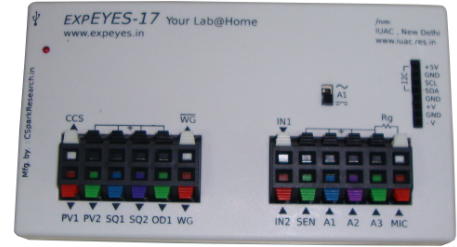
\includegraphics[scale = 0.7]{Figures/expeyes.png}
        \caption{expEYES kit}
        \label{fig:expeyes}
    \end{figure}

\section{Experiments}
    \subsection{Electromagnetic Induction}
    According to Faraday’s law of EM induction, whenever the flux linked with a coil changes, an emf is induced in the coil which is proportional to the rate of change of flux linkage. Also, Lenz’s law states that the emf is induced in such a direction as to oppose the change in flux. So this emf causes an eddy current to be developed in the coil. This emf is given by
    \begin{equation}
        \epsilon = -N \dfrac{d \Phi}{dt}
    \end{equation}
    according to Faraday’s law, where $\Phi$ the flux.
    \begin{equation}
    \label{eq:b/a}
        \epsilon = -N \dfrac{d (B/A)}{dt}
    \end{equation}
    where $A$ is the area of the coil, $N$ is the number of turns of the coil and $B$ is the magnetic field produced due to the small cylindrical bar magnet at the centre of the coil.
    \par
    Consider the case in which the magnet is moved through the coil with a constant velocity using some mechanism. We can consider the magnet with a dipole moment $m$ as a current-carrying loop having $n$ turns if the length of the magnet is appreciably small.
    \begin{equation}
    \label{eq:dipole}
        \begin{split}
            m &= nIA = n I \pi R^2 \\
            \implies nI R^2 &= \dfrac{m}{\pi}
        \end{split}
    \end{equation}
    where $R$ is the radius of the cylindrical magnet.
    \par
    We know that the field along the axis of the circular coil is given by
    \begin{equation}
    \label{eq:cirmag}
        B = \dfrac{\mu_0 n I R^2}{2} (R^2 +x^2)^{-3/2}
    \end{equation}
    where $x$ is the distance from the centre of the magnet to the centre of the coil. Using (\ref{eq:b/a}) and (\ref{eq:dipole}) and simplifying (\ref{eq:cirmag}), we get
    \begin{equation}
        \epsilon = \dfrac{3 \mu_0 m}{2 \pi} NA (R^2 +x^2)^{-5/2}xv
    \end{equation}
    If we drop the magnet vertically along the $z$-direction keeping the coil at origin, as shown in figure (\ref{fig:emdown}), gravity gets involved and we end up with the following equation
    \begin{equation}
        \begin{split}
            \epsilon = &\dfrac{3 \mu_0 m}{2 \pi} NA \Big( -z_0 + \dfrac{1}{2}gt^2 \Big) \\
            & \times \Bigg(R^2 + \Big( -z_0 + \dfrac{1}{2}gt^2 \Big)^2 \Bigg)^{-5/2} gt
        \end{split}
    \end{equation}
    If the magnet is long enough it cannot be considered as a simple coil, but should rather be considered as a solenoid with n turns. Since the magnet we are considering is a cylindrical magnet, it can be easily approximated as a solenoid.
    \begin{figure}
        \centering
        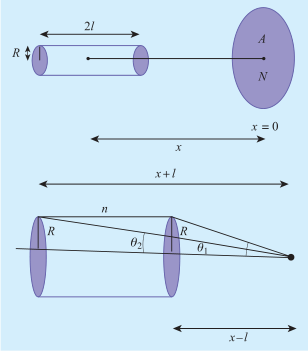
\includegraphics{Figures/longmagnet.png}
        \caption{A schematic representation of a long magnet moving horizontally through a coil.}
        \label{fig:longmagnet}
    \end{figure}
    The field along the axis of a solenoid is given by
    \begin{equation}
        \begin{split}
            B = &\dfrac{\mu_0 n_l I}{2} (\cos \theta_2 - \cos \theta_1) \\
            & =\dfrac{\mu_0 I n}{2 \times 2l} ((x+l) (R^2 + (x+l)^2)^{-1/2} \\
            & -(x-l)(R^2 + (x-l)^2)^{-1/2})
        \end{split}
    \end{equation}
    where $x$ is the distance from the centre of the coil to the centre of the magnet, as shown in figure (\ref{fig:longmagnet}). $l$ is the half length of the magnet, $R$ is the radius of the cylindrical magnet and $n_l (=n/2l)$ is the number of turns per unit length.
    \par
    If the magnet is falling vertically, let us take the direction of motion of the magnet to be in the positive $z$-direction, as shown in figure (\ref{fig:emdown}). Let the coil be at the origin $z = 0$ and the initial position of the magnet (the point at which we are dropping the magnet) be $-z_0$ at time $t = 0$. For this case, the emf induced is
    \begin{equation}
    \label{eq:finalem}
        \begin{split}
            \epsilon &= -\dfrac{NAm \mu_0}{4 \pi l} gt \Bigg[\Big(R^2 + \big(-z_0 + \frac{1}{2}gt^2 +l\big)^2 \Big)^{-3/2} \\
            & - \Big(R^2 + \big(-z_0 + \frac{1}{2}gt^2 -l\big)^2 \Big)^{-3/2} \Bigg]
        \end{split}
    \end{equation}
    \begin{figure}
        \centering
        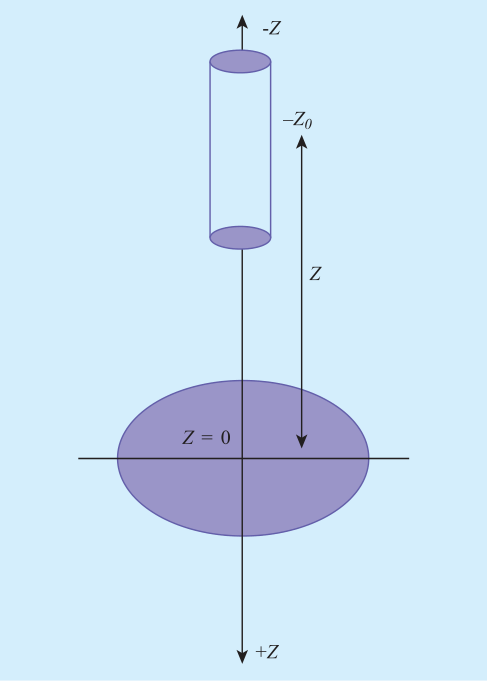
\includegraphics[scale = 0.65]{Figures/emInd.png}
        \caption{A schematic representation of a magnet falling vertically through a coil.}
        \label{fig:emdown}
    \end{figure}
    The schematic for the experiment is given in figure (\ref{fig:emschem}).
    \begin{figure}
        \centering
        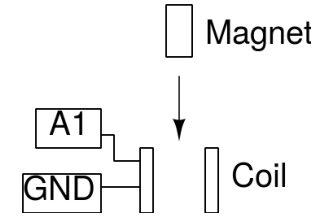
\includegraphics[scale = 0.6]{Figures/emSchematic.png}
        \caption{Schematic of the circuit for EM induction experiment through expEYES kit}
        \label{fig:emschem}
    \end{figure}
    \subsection{Opto-electric signal transmission}
    An opto-electronic oscillator (OEO) is an optoelectronic circuit that produces repetitive electronic sine wave and/or modulated optical continuous wave signals.
    \par
    A device called as phototransitor when illuminated by light at the base region, creates electron-hole pairs that modulate the base-collector junction resulting in an amplified current through transistor action. npn type transistor is used in this experiment. We will see how the intensity of light affects transistor action and also plot the output waveform from it.
    \begin{figure}
        \centering
        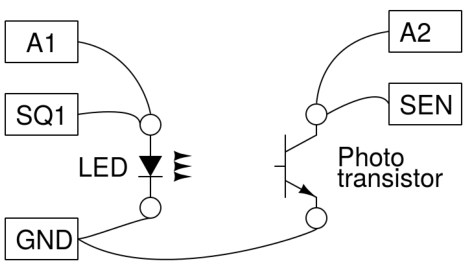
\includegraphics[scale = 0.5]{Figures/photoTra.png}
        \caption{Circuit for Phototransistor}
        \label{fig:photo}
    \end{figure}
    \subsection{IC555 Oscillator}
    There are three $\SI{5}{\kilo \ohm}$ resistors connected together internally producing a voltage divider network between the supply voltage at pin 8 and ground at pin 1 and hence the name 555 timers. The voltage across this series resistive network holds the negative inverting input of comparator two at $\frac{2}{3}V_{cc}$ and the positive non-inverting input to comparator one at $\frac{1}{3}V_{cc}$.The two comparators produce an output voltage dependent upon the voltage difference at their inputs. The outputs from both comparators are connected to the two inputs of the flip-flop which in turn produces either a 1 or 0 output based on the states of its inputs which controls a high current output switching stage to drive the connected load producing either a 1 or 0 voltage at the output pin.
    \par
    IC555 can be used as an a stable oscillator by connecting two resistors and a capacitor across its terminals to generate a fixed pulse with a time period determined by the time constant of the RC network.
    \par
    We will be measuring the duty cycle of rectangular pulse in this experiment. It is defined as the ratio of time for which the signal is in high state and the period of the signal.
    \begin{figure}
        \centering
        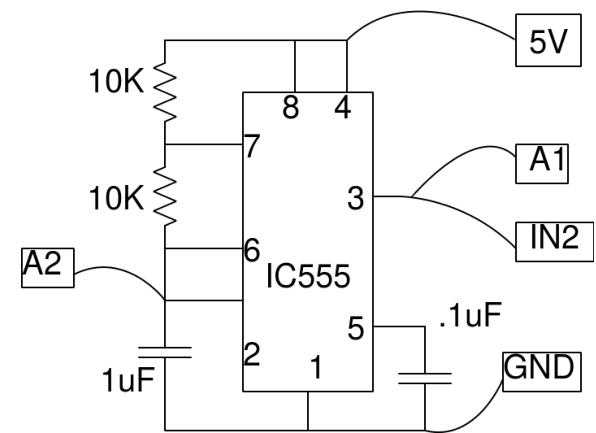
\includegraphics[scale = 0.45]{Figures/ic555.png}
        \caption{Circuit for IC555 timer}
        \label{fig:ic555}
    \end{figure}
    \par
    The frequency can be calculated using the formula
    \begin{equation}
    \label{eq:freq}
        f = \dfrac{1}{\ln 2 \times C \times (R_1 + 2R_2)}
    \end{equation}
    The HIGH TIME is given by
    \begin{equation}
    \label{eq:high}
        t_H = \ln 2 \times C \times (R_1 + 2R_2)
    \end{equation}
    and the LOW time is given by
    \begin{equation}
    \label{eq:low}
        t_L = \ln 2 \times C \times R_2
    \end{equation}
\section{Observations, graphs and calculations}
    \subsection{Electromagnetic Induction}
    The following observations were made
    \begin{enumerate}
        \item Coil diameter, $D_{coil} = \SI{1.29}{\centi \metre}$,
        \item Tube length, $2z_0 = \SI{21}{\centi \metre}$.
        \item Number of turns in the coil, $N = 3000$,
        \item Length of the magnet $l = \SI{0.98}{\centi \metre}$,
        \item Diameter of the magnet, $D_{magnet} = \SI{0.29}{\centi \metre}$
    \end{enumerate}
    \begin{figure}
        \centering
        \begin{subfigure}[b]{0.5\textwidth}
            \centering
            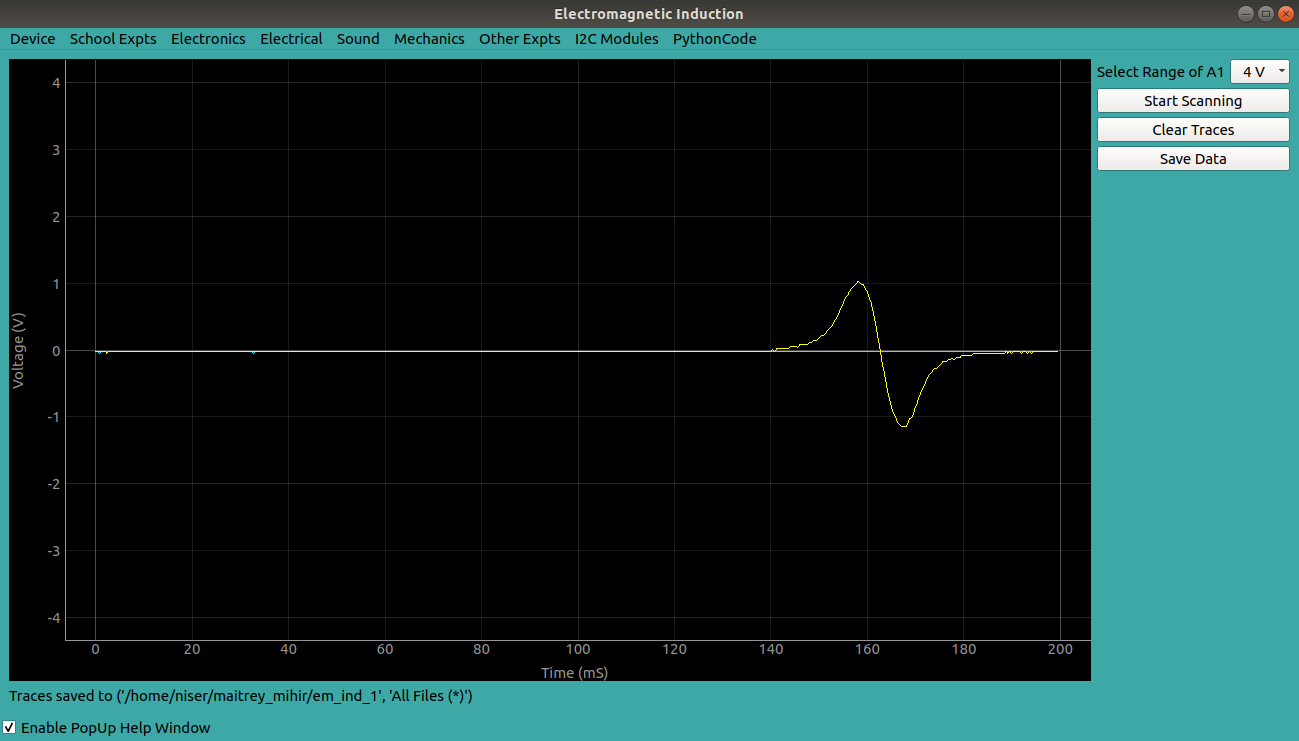
\includegraphics[scale = 0.19]{Figures/em_ind_1.png}
        \end{subfigure}
        \hfill
        \begin{subfigure}[b]{0.5\textwidth}
            \centering
            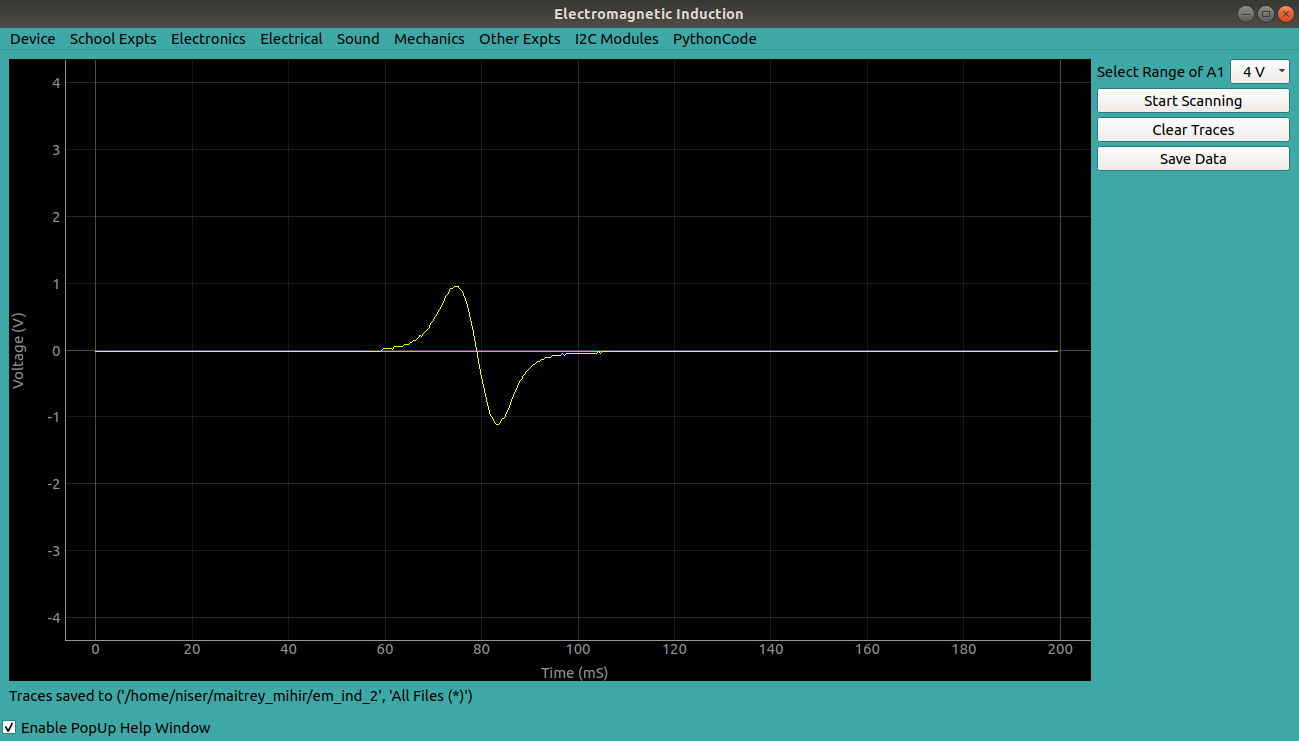
\includegraphics[scale = 0.19]{Figures/em_ind_2.png}
            \caption{The above two figures show the pulse of emf as magnet falls down}
            \label{fig:em2}
        \end{subfigure}
        \hfill
        \begin{subfigure}[b]{0.5\textwidth}
            \centering
            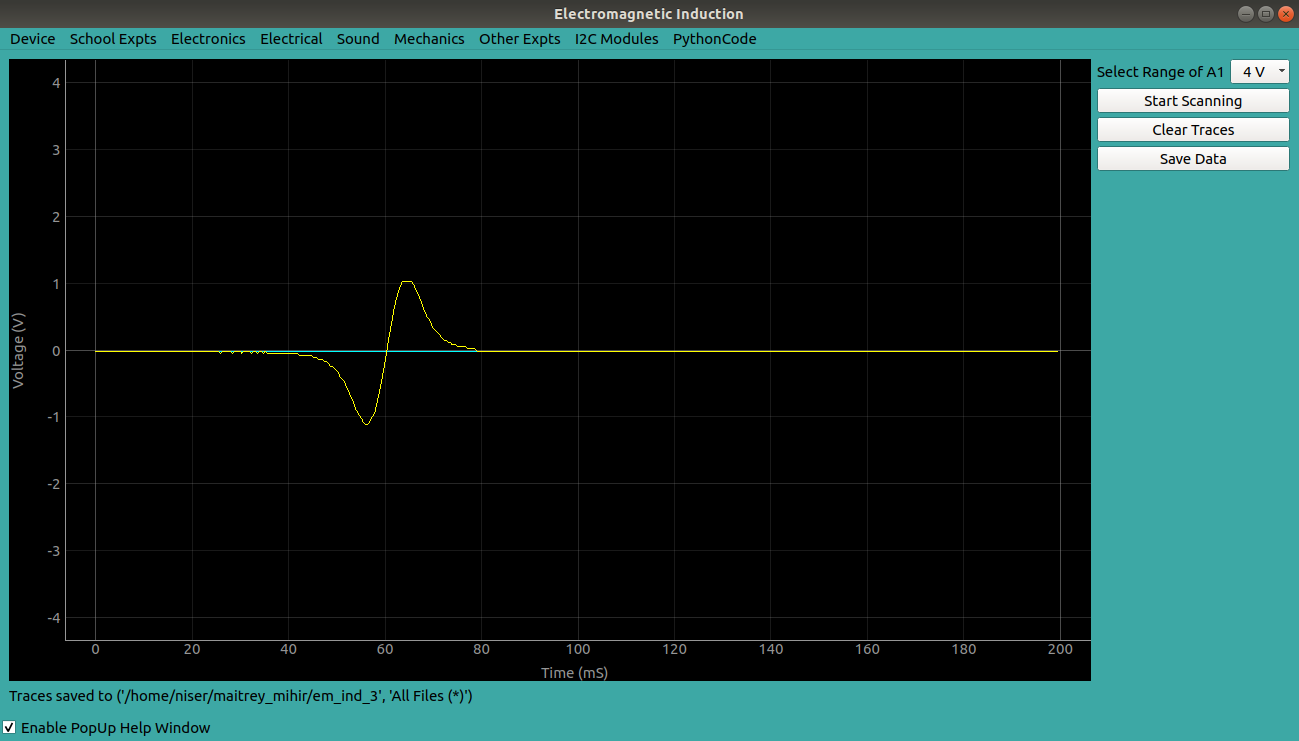
\includegraphics[scale = 0.19]{Figures/em_ind_3.png}
            \caption{Similar result is obtained, albeit with flipped polarity as we change the direction of magnet as it is thrown down}
            \label{fig:em3}
        \end{subfigure}
            \caption{emf induced in the coil as a result of magnet passing through it}
            \label{fig:em}
    \end{figure}
    \begin{figure}[h!]
        \centering
        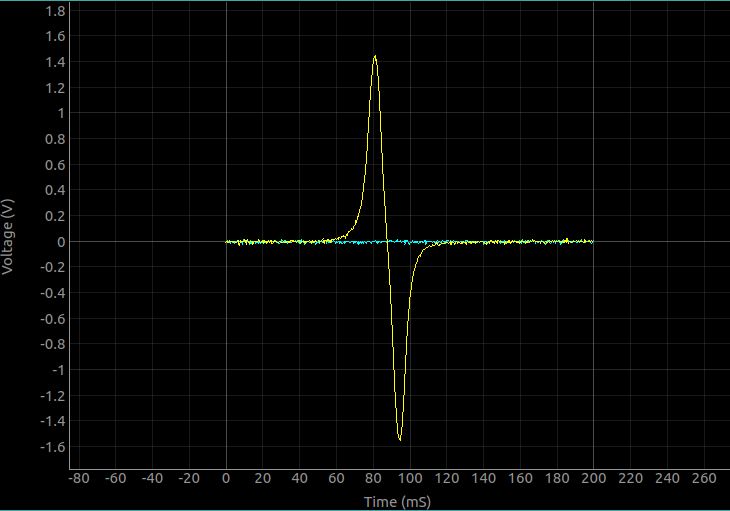
\includegraphics[scale = 0.25]{Figures/two magnet normal 22.2 mid ie 11.1.png}
        \caption{emf induced for the case when magnets joined were dropped through the coil}
        \label{fig:twomag}
    \end{figure}
    \subsubsection{For a single magnet}
    Time taken to pass through the coil was $t = \SI{0.062}{\second}$ and emf induced was $\epsilon = \SI{0.952}{\volt}$. Using equation (\ref{eq:finalem}), we get $m = \SI{91.1}{\ampere \per \metre \squared}$.
    \subsubsection{For two magnets joined}
    Time taken to pass through the coil was $t = \SI{0.044}{\second}$ and emf induced was $\epsilon = \SI{1.456}{\volt}$. Using equation (\ref{eq:finalem}), we get $m = \SI{288.9}{\ampere \per \metre \squared}$.
    \subsection{Opto-electric signal transmission}
    We observe the change in the voltage across the phototransistor (green pulse). The square trace is the voltage across the LED. the yellow square pulse was fed in at $\SI{1}{\kilo \hertz}$ and the green plot was the phototransistor response.
    \begin{figure*}[htp]
    \centering
    \begin{tabular}{cccc}
    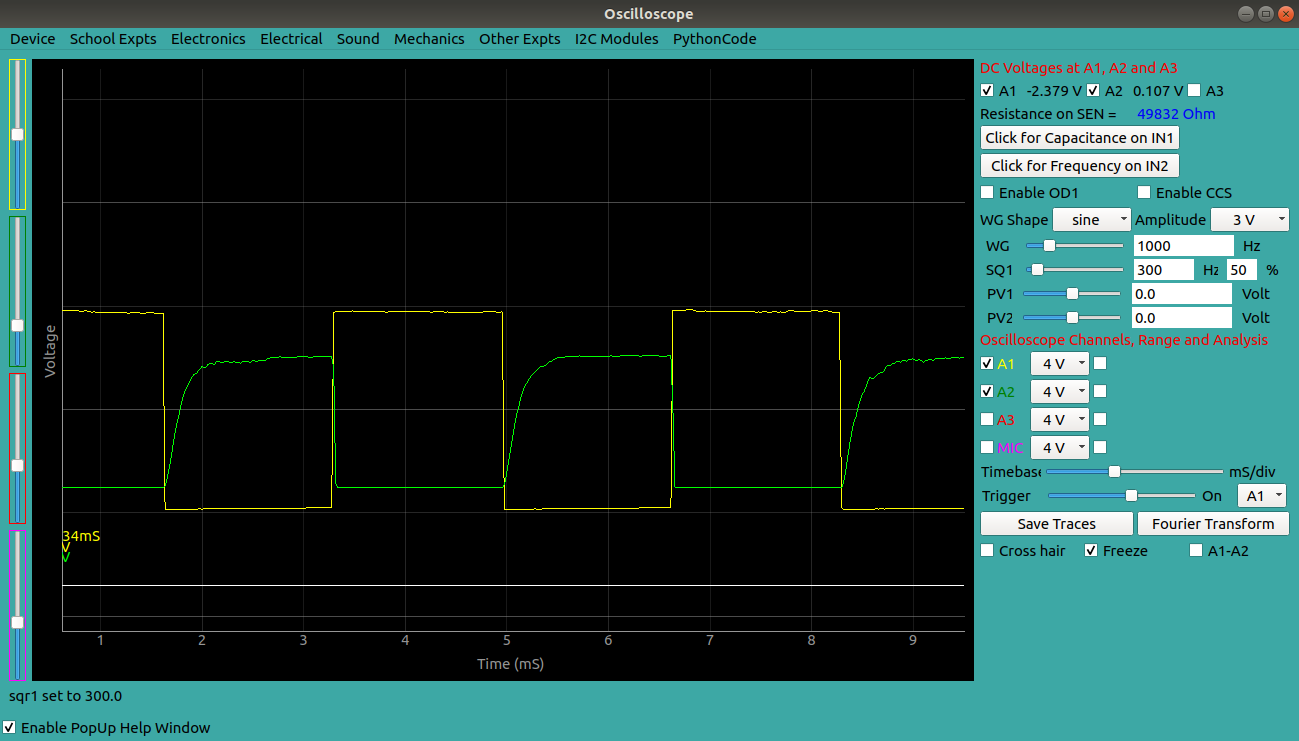
\includegraphics[width=.325\textwidth]{Figures/photo_300.png} &
    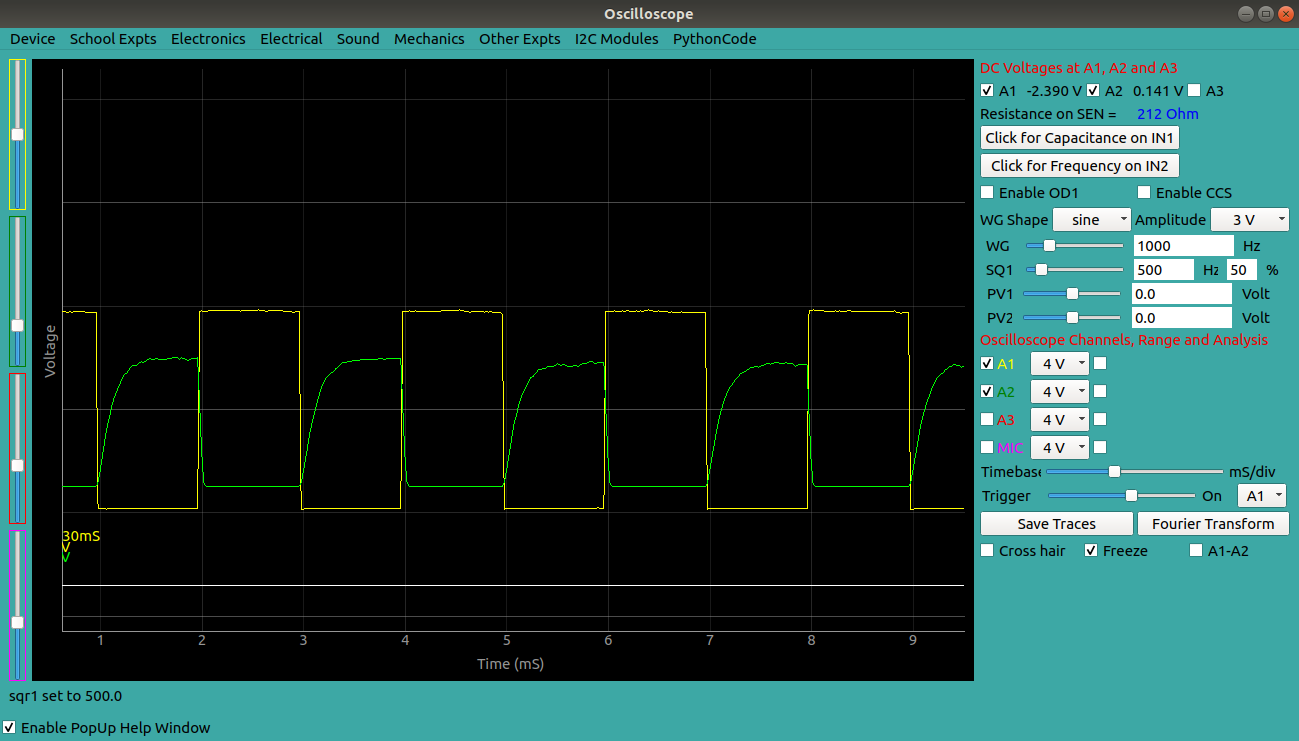
\includegraphics[width=.325\textwidth]{Figures/phto_500.png} &
    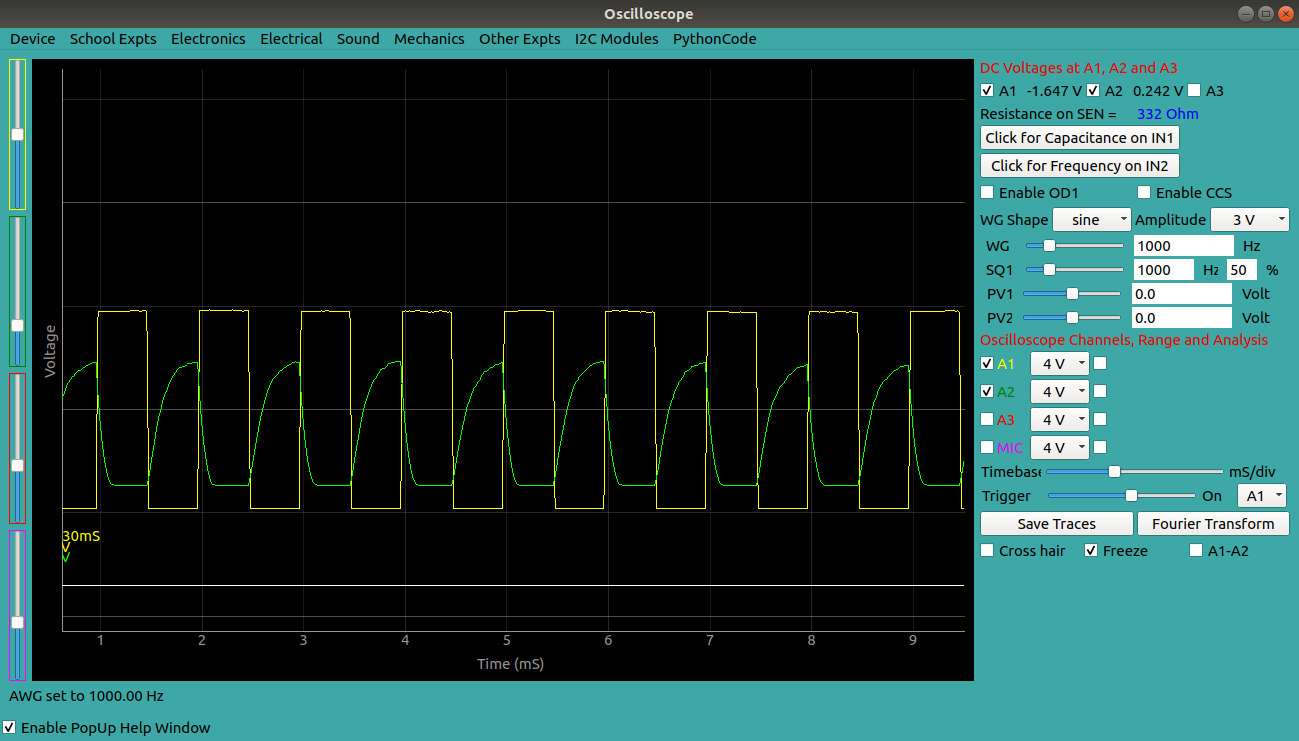
\includegraphics[width=.325\textwidth]{Figures/photo_1000.png} \\
    (a) $\SI{300}{\hertz}$ & (b) $\SI{500}{\hertz}$ & (c) $\SI{1000}{\hertz}$  \\[6pt]
    \end{tabular}
    \medskip
    \begin{tabular}{cccc}
    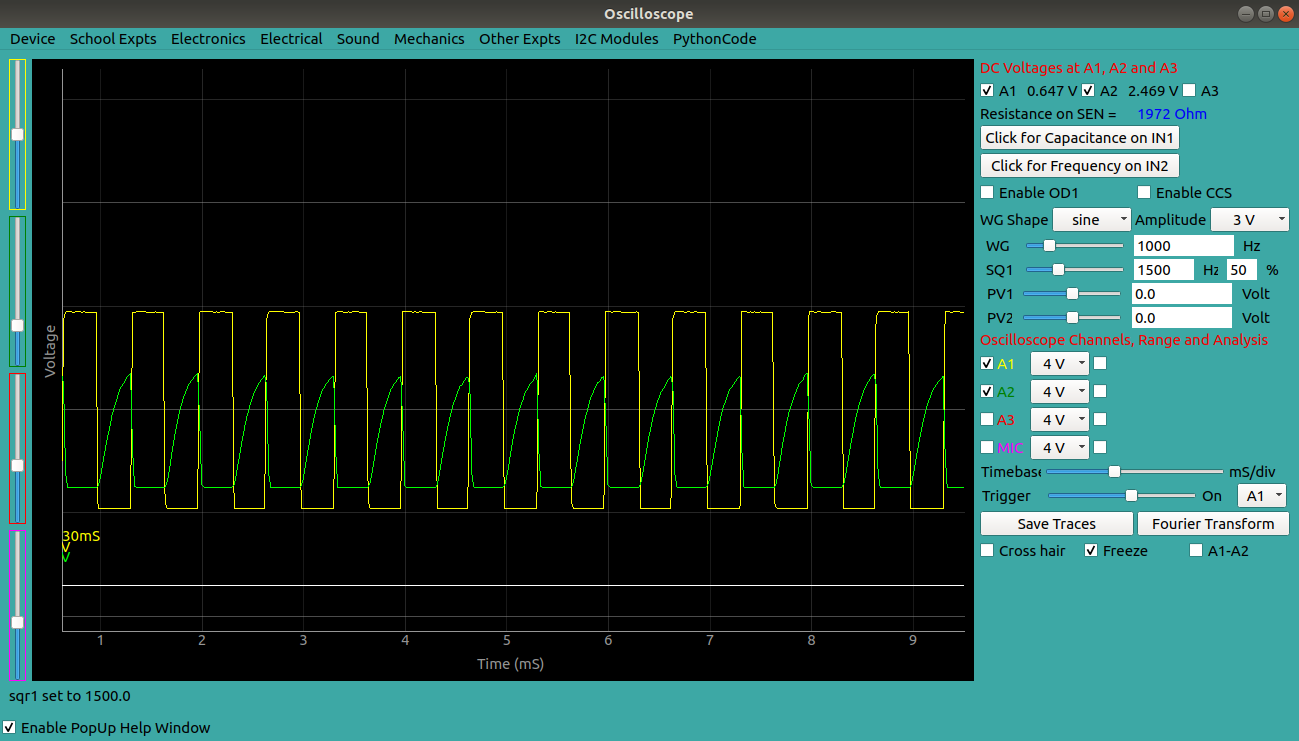
\includegraphics[width=.325\textwidth]{Figures/photo_1500.png}&
    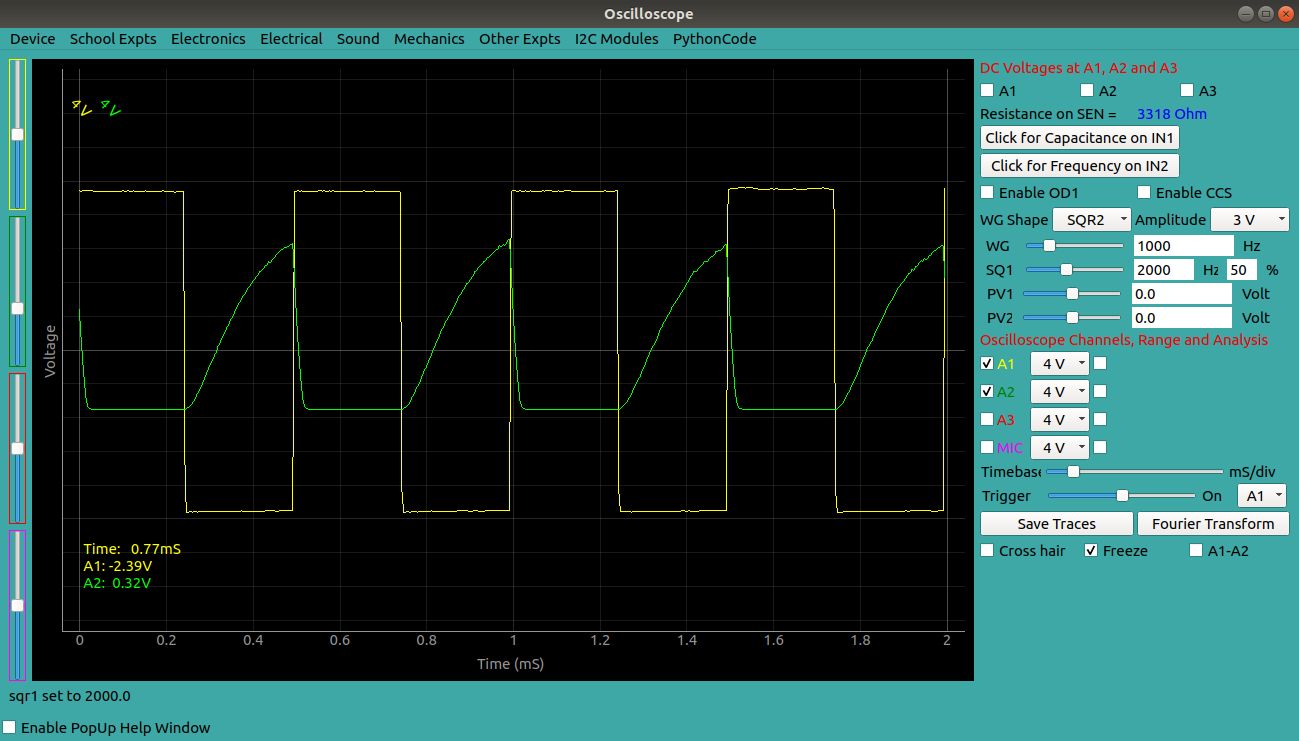
\includegraphics[width=.325\textwidth]{Figures/photo_2000.png}&
    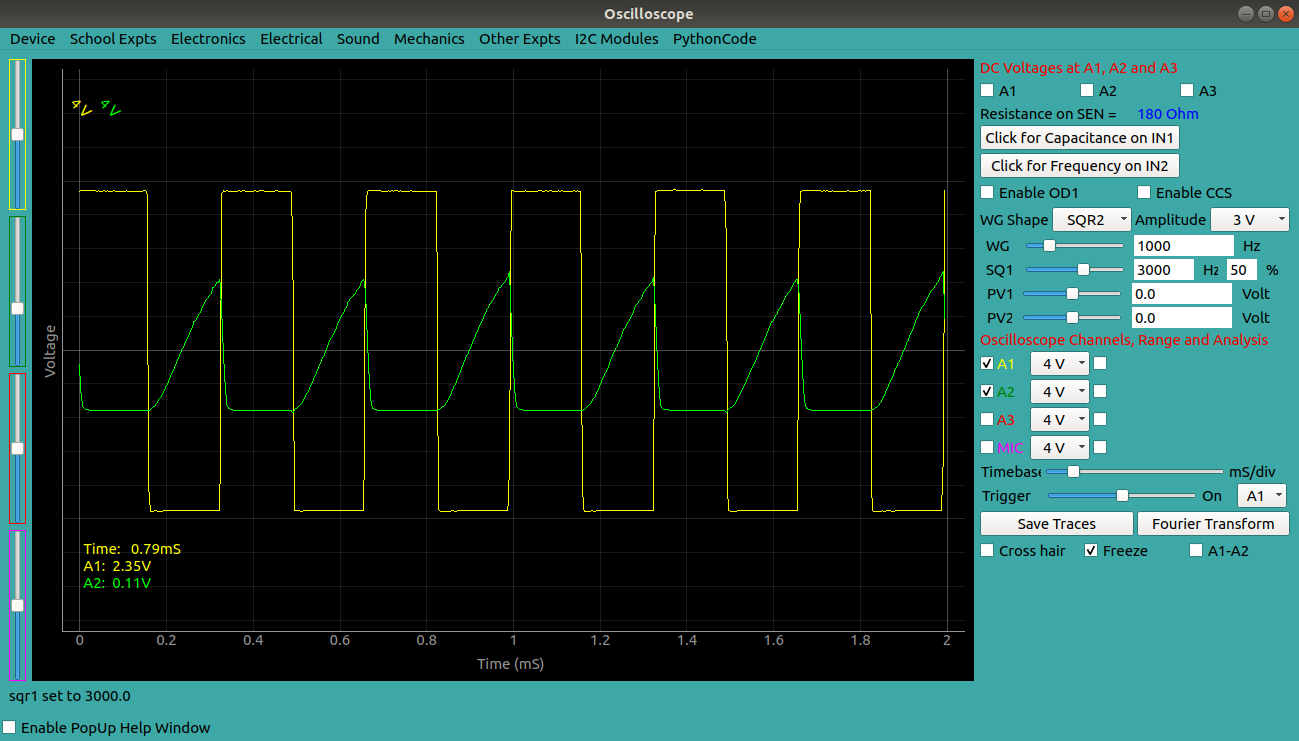
\includegraphics[width=.325\textwidth]{Figures/photo_3000.png}\\
    (d) $\SI{1500}{\hertz}$ & (e) $\SI{2000}{\hertz}$ & (f) $\SI{3000}{\hertz}$  \\[6pt]
    \end{tabular}
    \caption{Graphs obtained for opto-electric signal transmission experiment through phototransistor}
    \label{fig:opto}
    \end{figure*}
    \subsection{IC555 Oscillator}
    There were three combinations studied for the IC555 oscillator:
    \begin{enumerate}
        \item $R_1 = \SI{1}{\kilo \ohm}$, $R_2 = \SI{10}{\kilo \ohm}$
        Using equation (\ref{eq:freq}), we get $f = \SI{68.65}{\kilo \hertz}$. The observed frequency was $\SI{48.6}{\kilo \hertz}$. HIGH and LOW times were found using equations (\ref{eq:high}) and (\ref{eq:low}) respectively as $t_H = \SI{7.6e-3}{\second}$ and $t_L = \SI{6.93e-3}{\second}$.
        \par
        From here duty cycle can be calculated as
        \begin{equation}
            \text{Duty cycle} = \dfrac{t_H}{t_H + t_L} \times 100 \% = 52.3 \%
        \end{equation}
        The observed duty cycle was $67.8 \%$
        \item $R_1 = \SI{2}{\kilo \ohm}$, $R_2 = \SI{10}{\kilo \ohm}$
        Using equation (\ref{eq:freq}), we get $f = \SI{68.58}{\kilo \hertz}$. The observed frequency was $\SI{66.8}{\kilo \hertz}$. HIGH and LOW times were found using equations (\ref{eq:high}) and (\ref{eq:low}) respectively as $t_H = \SI{8.3e-3}{\second}$ and $t_L = \SI{6.93e-3}{\second}$.
        \par
        From here duty cycle can be calculated as
        \begin{equation}
            \text{Duty cycle} = \dfrac{t_H}{t_H + t_L} \times 100 \% = 54.5 \%
        \end{equation}
        The observed duty cycle was $54.9 \%$.
        \item $R_1 = \SI{10}{\kilo \ohm}$, $R_2 = \SI{10}{\kilo \ohm}$
        Using equation (\ref{eq:freq}), we get $f = \SI{48.08}{\kilo \hertz}$. The observed frequency was $\SI{36.3}{\kilo \hertz}$. HIGH and LOW times were found using equations (\ref{eq:high}) and (\ref{eq:low}) respectively as $t_H = \SI{1.39e-2}{\second}$ and $t_L = \SI{6.93e-3}{\second}$.
        \par
        From here duty cycle can be calculated as
        \begin{equation}
            \text{Duty cycle} = \dfrac{t_H}{t_H + t_L} \times 100 \% = 66.73 \%
        \end{equation}
        The observed duty cycle was $65 \%$.
    \end{enumerate}
    \begin{figure}
        \centering
        \begin{subfigure}[b]{0.5\textwidth}
            \centering
            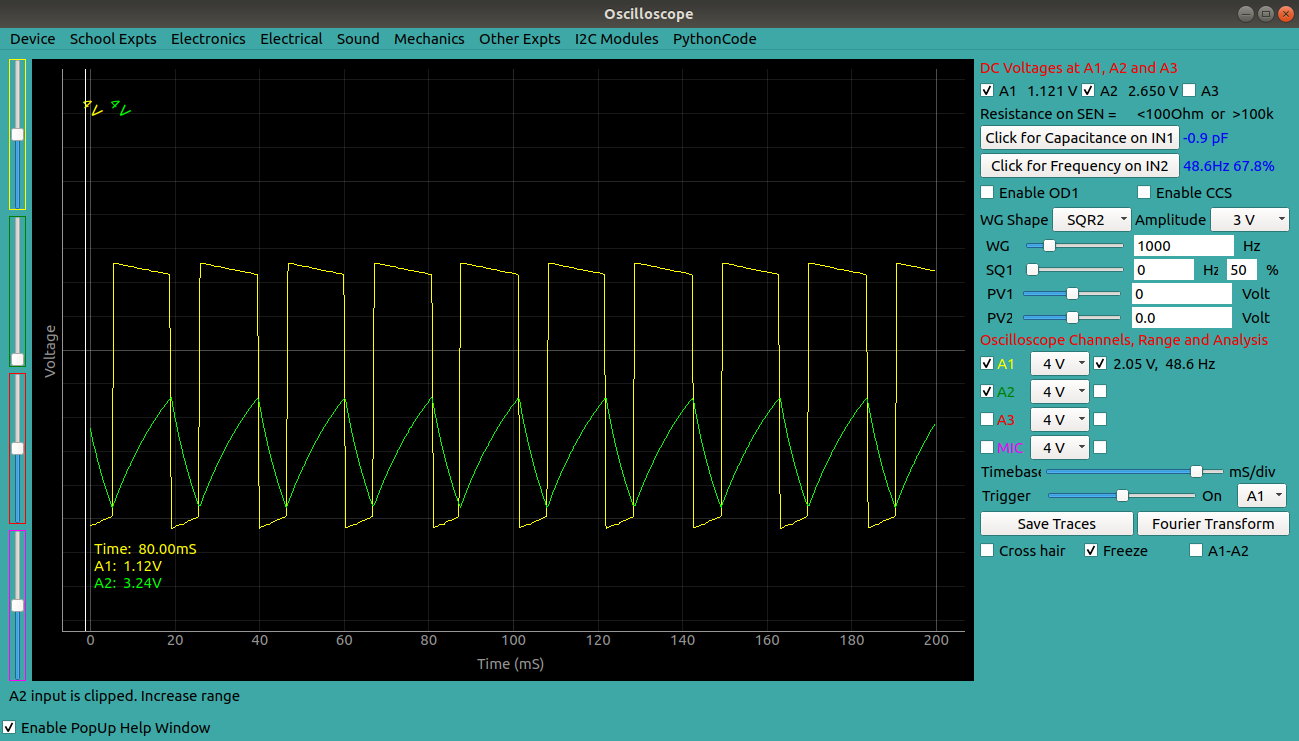
\includegraphics[scale = 0.19]{Figures/ic555_1,10.png}
            \caption{IC555 oscillator results for $R_1 = \SI{1}{\kilo \ohm}$, $R_2 = \SI{10}{\kilo \ohm}$}
            \label{fig:90spec}
        \end{subfigure}
        \hfill
        \begin{subfigure}[b]{0.5\textwidth}
            \centering
            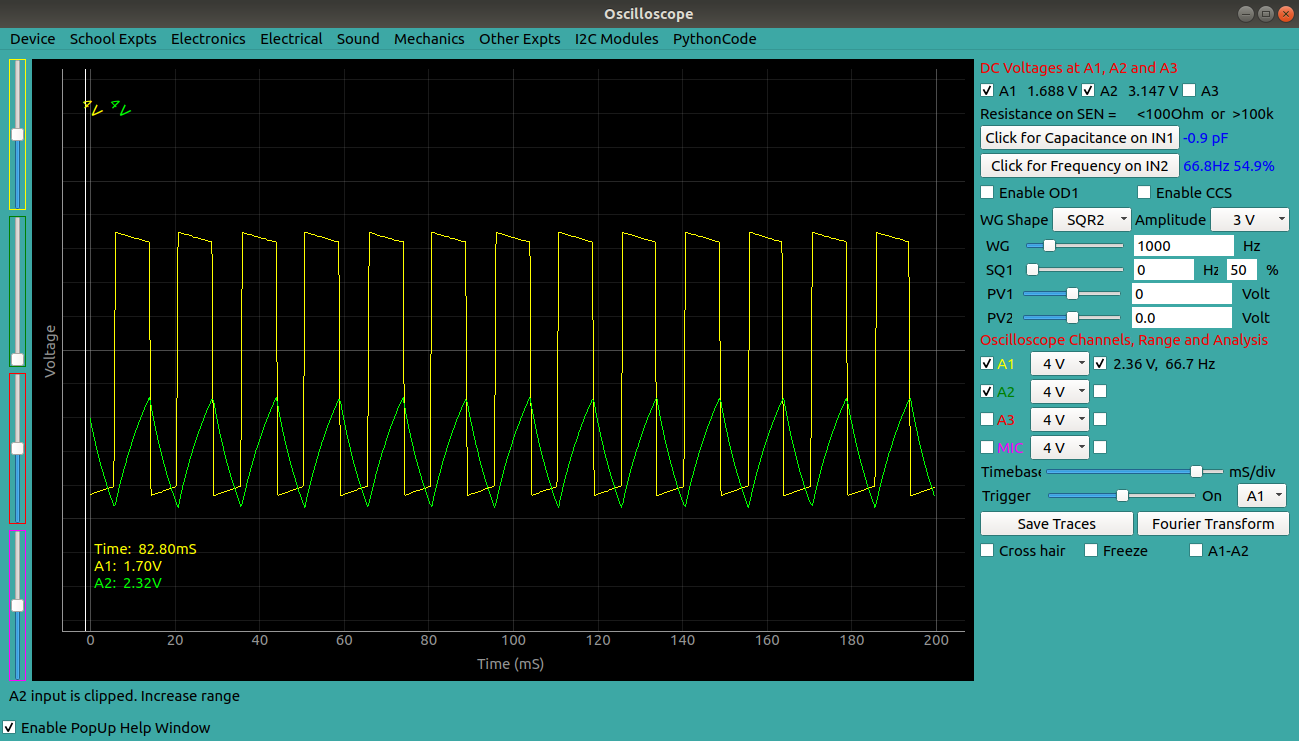
\includegraphics[scale = 0.19]{Figures/ic555_2,10.png}
            \caption{IC555 oscillator results for $R_1 = \SI{2}{\kilo \ohm}$, $R_2 = \SI{10}{\kilo \ohm}$}
            \label{fig:90gate}
        \end{subfigure}
        \hfill
        \begin{subfigure}[b]{0.5\textwidth}
            \centering
            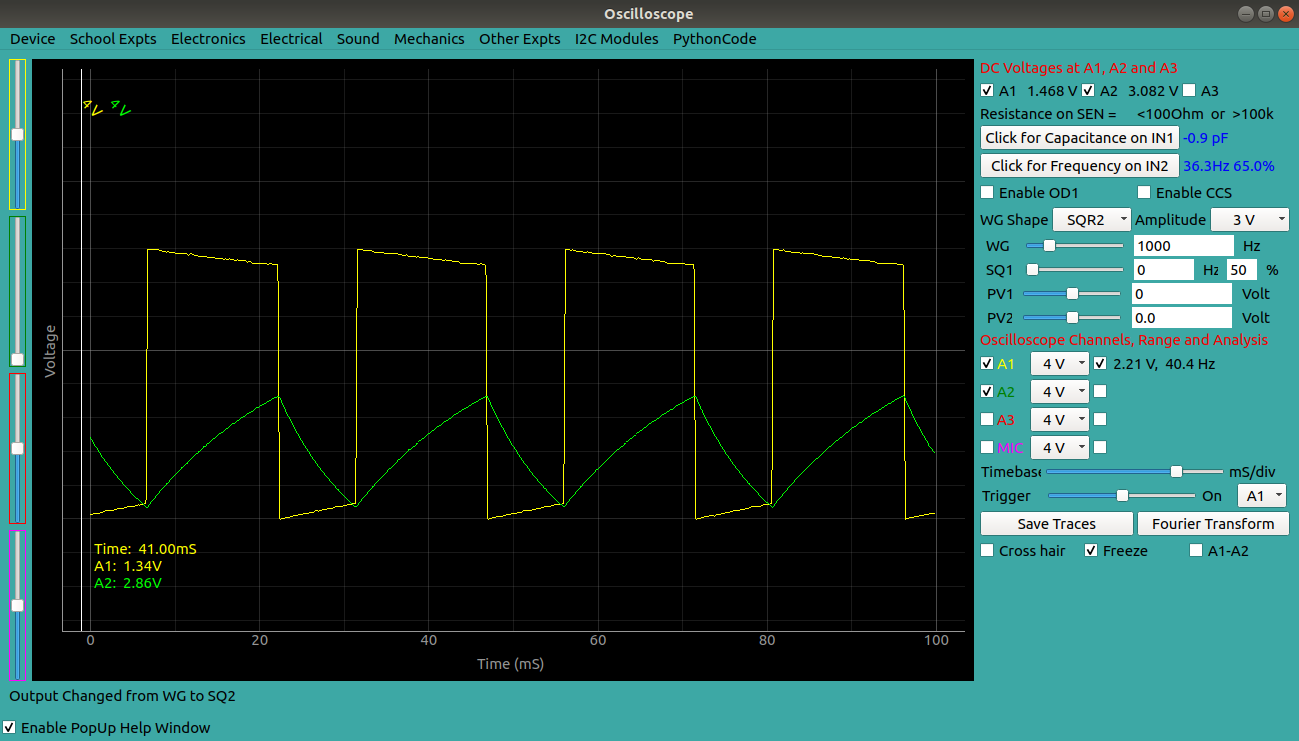
\includegraphics[scale = 0.19]{Figures/ic555_10,10.png}
            \caption{IC555 oscillator results for $R_1 = \SI{10}{\kilo \ohm}$, $R_2 = \SI{10}{\kilo \ohm}$}
            \label{fig:90gate}
        \end{subfigure}
            \caption{Graphs obtaned for IC555 experiment}
            \label{fig:90}
    \end{figure}
\section{Error Analysis}
\subsection{Electromagnetic Induction}
\subsubsection{For a single magnet}
    \begin{equation}
        \dfrac{\delta m}{m} = \sqrt{\dfrac{1}{3}\Big(\dfrac{dR}{R}\Big)^2+\dfrac{1}{3}\Big(\dfrac{dl}{l}\Big)^2+\dfrac{1}{3}\Big(\dfrac{dz}{z}\Big)^2}
    \end{equation}
    From here we get $\delta m = \SI{1.3}{\ampere \per \metre \squared}$.
    \subsubsection{For two magnets joined}
    \begin{equation}
        \dfrac{\delta m}{m} = \sqrt{\dfrac{1}{3}\Big(\dfrac{dR}{R}\Big)^2+\dfrac{1}{3}\Big(\dfrac{dl}{l}\Big)^2+\dfrac{1}{3}\Big(\dfrac{dz}{z}\Big)^2}
    \end{equation}
    From here we get $\delta m = \SI{3.3}{\ampere \per \metre \squared}$.
    
\section{Results}
    \begin{enumerate}
        \item The magnetic moment for a single magnet was obtained as $m_1 =  \SI[separate-uncertainty=true]{91.1\pm 1.3}{\ampere \per \metre \squared}$, and for two magnets joined, the magnetic moment was obtained as $m_2 = \SI[separate-uncertainty=true]{288.9\pm 3.3}{\ampere \per \metre \squared}$
        \item For $R_1 = \SI{1}{\kilo \ohm}$, $R_2 = \SI{10}{\kilo \ohm}$, the observed frequency was $\SI{48.6}{\kilo \hertz}$ and the calculated frequency was $\SI{68.65}{\kilo \hertz}$. observed duty cycle was $67.8\%$ while the calculated duty cycle was $52.3 \%$. The calculated HIGH and LOW times were $t_H = \SI{7.6e-3}{\second}$ and $t_L = \SI{6.93e-3}{\second}$.
        \item For $R_1 = \SI{2}{\kilo \ohm}$, $R_2 = \SI{10}{\kilo \ohm}$, the observed frequency was $\SI{66.8}{\kilo \hertz}$ and the calculated frequency was $\SI{65.58}{\kilo \hertz}$. observed duty cycle was $54.9\%$ while the calculated duty cycle was $54.5 \%$. The calculated HIGH and LOW times were $t_H = \SI{8.3e-3}{\second}$ and $t_L = \SI{6.93e-3}{\second}$.
        \item For $R_1 = \SI{10}{\kilo \ohm}$, $R_2 = \SI{10}{\kilo \ohm}$, the observed frequency was $\SI{36.6}{\kilo \hertz}$ and the calculated frequency was $\SI{48.08}{\kilo \hertz}$. observed duty cycle was $65\%$ while the calculated duty cycle was $67.3 \%$. The calculated HIGH and LOW times were $t_H = \SI{1.39e-2}{\second}$ and $t_L = \SI{6.93e-3}{\second}$.
    \end{enumerate}

\section{Discussions}
    \begin{enumerate}
        \item We obtained 2 peaks in opposite directions from our reference axis. This is because due to Lenz's law first the rate of change of flux result in positive peak but once the flux is maximum then the rate of change of flux is opposite in sign because the magnet is now receding from the center. At the center of the tube, the EMF is 0. The positive peak of induced EMF does not coincide exactly with a quarter length of the tube; it is slightly shifted to the right. This is due to gravitational force. The negative peak is higher than the positive peak because the velocity is higher when the second peak is plotted.
        \item During the entry, the emf induced is positive and while exiting it is negative as it can be seen from the graph (figure (\ref{fig:em2})). It changed when the magnet is thrown after changing its orientation (\ref{fig:em3}), as expected.
        \item The emf induced when two magnets are joined together was more as expected.
        \item The graphs so plotted for the incident light and the photo response were found to be out of phase. This is because when a current $I_B$ is applied to base, an output appears across the collector-emitter junction. So, no voltage is dropped across the LED and it doesn’t glow. When $I_B$ is zero (low region of square pulse), all input voltage is dropped across the LED, thereby making it glow.
        \item Due to presence of capacitors in the circuits of phototransistor and IC555 timer; exact square pulses were not obtained. In IC555, capacitors are actually present in the circuit, while in the base region of phototransistor, electron-hole generation creates the capacitance type of effect. In low frequency signal however, the output becomes nearly a perfect square wave.
    \end{enumerate}

\section{Conclusions}
    \begin{enumerate}
        \item Using a current induced coil and a magnet, we successfully performed electromagnetic induction experiment.
        \item We were also successful in performing the phototransistor experiment and the obtained response has been attached.
        \item We operated IC555 timer in astable multivibrator mode and observed and calculated the duty cycle and frequency of the wave for three different combination of resistors.
        \item We learned the application of ExpEYES kit as a function generator, oscilloscope and as voltmeter.
    \end{enumerate}
    
\section{Precautions}
\begin{enumerate}
    \item The magnet should fall straight through the tube avoiding any collisions.
    \item Inputs A1 and A2 must be within ±16 volts range and Inputs IN1 and IN2 must be in 0 to 3.3V range. To measure higher voltages, scale them down using resistive potential divider networks.
    \item Be careful of loose connections.
\end{enumerate}

\end{document}
%
% ****** End of file aipsamp.tex ******